\documentclass[9pt]{beamer}

\usetheme[{titleformat plain}=smallcaps,
           titleformat title=smallcaps,
           titleformat subtitle=regular,
           titleformat section=smallcaps,
           titleformat frame=smallcaps,
           numbering=fraction,
          ]{metropolis}
\usepackage{appendixnumberbeamer}
\geometry{paperwidth=213.3mm,paperheight=120mm}

\usepackage{../_style/common}
\usepackage{../_style/defs}
\usepackage{emoji}

\graphicspath{{pictures/}{../_pictures/}}

\title{Data and Interfaces}
\subtitle{
    \itshape
    successful abstractions as building blocks
}
\date{October, 2022}
\author{Alessandro Candido}
\titlegraphic{
    \vfill\vspace*{250pt}
    
\includegraphics[height=1cm]{../_logos/unimi_logo.png}\hfill
    
\includegraphics[height=1cm]{../_logos/infn_logo.png}\\
}

\begin{document}

\maketitle

\setlist[description]{font=\quad\normalfont\bfseries\scshape\space}
\metroset{block=fill}


\begin{frame}{Who am I?}
    \begin{columns}
        \begin{column}{0.5\textwidth}
            I am a \textbf{PhD student} in \textbf{HEP theory}, about to
            finish.\newline

            Since my Master I have spent a significant part of my research
            working on \alert{\textbf{software projects}}, with an increasing
            number of collaborators.\newline

            \vspace*{5pt}
            \partitle{References}
            \vspace*{5pt}

            Now, as part of \nnpdf{}, I had to work and organize projects with
            $\order{5\text{-}10}$ developers -- not incredibly many, but already
            \textit{\textbf{challenging}}.\newline

            Moreover, personal projects driven me to explore beyond the
            boundaries of what is useful for physics.
            With less \sout{pressure} needs you can explore more\dots but often
            not as deep.\newline

            \vspace*{5pt}
            \partitle{My Goal}
            \vspace*{5pt}

            I am not here to teach, but just to \textbf{share my experience}.
            This is compliant with the references.
        \end{column}
        \begin{column}{0.5\textwidth}
            \begin{figure}
                \centering
                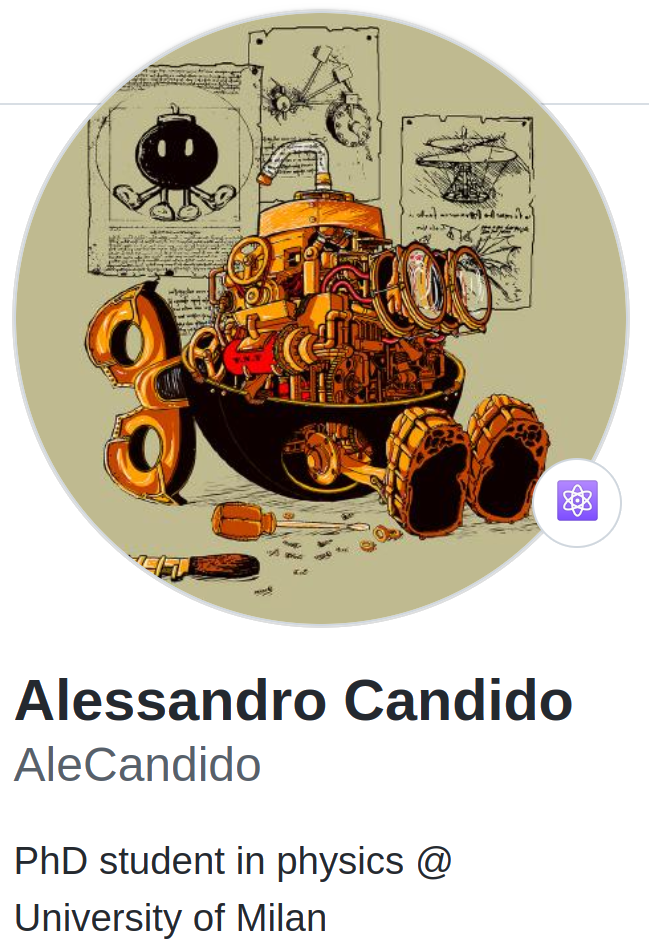
\includegraphics[width=0.5\textwidth]{mygh}
            \end{figure}
        \end{column}
    \end{columns}
\end{frame}

% \begin{frame}{The Role of Trade-offs}
    % \begin{columns}
        % \begin{column}{0.5\textwidth}
            % \vspace*{20pt}
            % \begin{center}
                % \itshape\bfseries 
                % There are no absolute truths.
            % \end{center}
            % \begin{flushright}
                % \itshape
                % -- is this an absolute truth? \emoji{thinking-face}
            % \end{flushright}

            % \vspace*{10pt}
            % In a sense, problems might look similar, even when they are not
            % that much\dots
            % \vspace*{20pt}
            
            % \begin{figure}
                % \centering
                % 
\includegraphics[width=\textwidth]{solution}
                % \caption{
                    % Artistic view of the solution function, over the space of
                    % problems.
                % }
            % \end{figure}
        % \end{column}
        % \begin{column}{0.5\textwidth}
            % So, better to know many possible solutions, and always consider
            % multiple alternatives.

            % \vspace*{10pt}
            % \begin{figure}
                % \centering
                % 
\includegraphics[width=0.6\textwidth]{balancing}
            % \end{figure}
            % \vspace*{10pt}

            % Moreover
            % \href{https://en.wikipedia.org/wiki/All_that_glitters_is_not_gold\#In_popular_culture}{\enquote{All
            % that is gold does not glitter}}, not all good solutions are
            % manifest.
        % \end{column}
    % \end{columns}
% \end{frame}

\begin{frame}{Outline}
    \vspace*{10pt}
    \begin{center}
        \itshape
        The task I have been given is to discuss \textbf{interfaces} and
        \textbf{data management.}
    \end{center}
    \vspace*{10pt}

    \begin{columns}
        \begin{column}{0.5\textwidth}
            \alert{\textbf{Python}} is not the \enquote{best} programming
            language, nor the unique one.
            But Python is definitely a successful one.
            \vspace*{10pt}

            And the success for a language is mostly determined by the
            availability of \textbf{libraries} and
            \textbf{applications}\footnote{
                There are relevant and determinant language features, and for
                Python is its \textbf{expressiveness}, that is fundamental for
                new users and \textit{\textbf{maintainability}}.
            }.\newline

            In the case of Python:
            \begin{description}
                \item[application] scientific computation, and data science\footnote{
                    Part of the success has been due to \textit{web
                    frameworks}, but it is less relevant nowadays.
                }
                \item[libraries] Numpy, Scipy, Pandas, Xarray, \dots
            \end{description}
            \vspace*{30pt}

            Of course ML frameworks now play a big a role, but it is almost a
            consequence\dots
            \vspace*{5pt}
        \end{column}
        \begin{column}{0.5\textwidth}
            So, in a sense, the advantage of Python is that its
            \alert{\textbf{libraries}} can be \alert{\textbf{written not in
            Python}}.

            But in order this to be possible, it is crucial to build a
            successful \textbf{abstraction}.
            \vspace*{20pt}

            \begin{enumerate}
                \item abstractions
                \item interfaces
                \item examples
                \item project management
            \end{enumerate}
            \vspace*{20pt}

            \begin{figure}
                \centering
                
\includegraphics[height=0.15\textwidth]{python}
                \hspace*{20pt}
                
\includegraphics[height=0.15\textwidth]{numpy}
                \hspace*{20pt}
                
\includegraphics[height=0.15\textwidth]{pandas}
                \hspace*{20pt}
                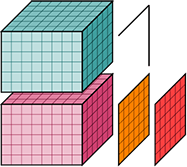
\includegraphics[height=0.15\textwidth]{xarray}
            \end{figure}
            \vspace*{10pt}
        \end{column}
    \end{columns}
\end{frame}

\section{Abstraction}

\begin{frame}{Template}
    \begin{columns}
        \begin{column}{0.5\textwidth}
            
        \end{column}
        \begin{column}{0.5\textwidth}
            
        \end{column}
    \end{columns}
\end{frame}

\section{Interfaces}

\begin{frame}{Template}
    \begin{columns}
        \begin{column}{0.5\textwidth}
            
        \end{column}
        \begin{column}{0.5\textwidth}
            
        \end{column}
    \end{columns}
\end{frame}

\section{Examples}

\begin{frame}{Template}
    \begin{columns}
        \begin{column}{0.5\textwidth}
            
        \end{column}
        \begin{column}{0.5\textwidth}
            
        \end{column}
    \end{columns}
\end{frame}

\section{Project Management}

\begin{frame}{Docs}
    \begin{center}
        Presenting the code is fundamental: since you \textbf{want to have
        users}, it has to be \textit{useful} and \textit{simple}.

        \textit{And everything is \textbf{simple, when} it is
        \alert{\textbf{well explained}}.}
    \end{center}
    \vspace*{10pt}

    \begin{columns}
        \begin{column}{0.35\textwidth}
            It is a synthetic replacement for office hours.
            \vspace*{10pt}

            \begin{itemize}
                \item given a \textbf{question}, the \textbf{answer} should be
                  properly written in the docs; in familiar terms, and simple
                  to find, not only: 
                \item sometimes, it should provide \textbf{answers before
                  questions} (since it is not always clear which are the proper
                  ones)
            \end{itemize}

            \begin{figure}
                \centering
                
\includegraphics[width=0.6\textwidth]{question-docs}
            \end{figure}
        \end{column}
        \begin{column}{0.35\textwidth}
            Good documentation have to provide resources for different users,
            so they need to be \textbf{hierarchical}.
            \vspace*{10pt}

            \begin{description}
                \item[presentation] a \textbf{home page}, to meet new users,
                    and a starting point
                \item[getting started] \textbf{tutorials}, to begin hands on
                \item[user manual] to answer most of the common needs
                \item[reference] a complete explanation of the public interface
            \end{description}
        \end{column}

        \begin{column}{0.3\textwidth}
            \begin{figure}
                \centering
                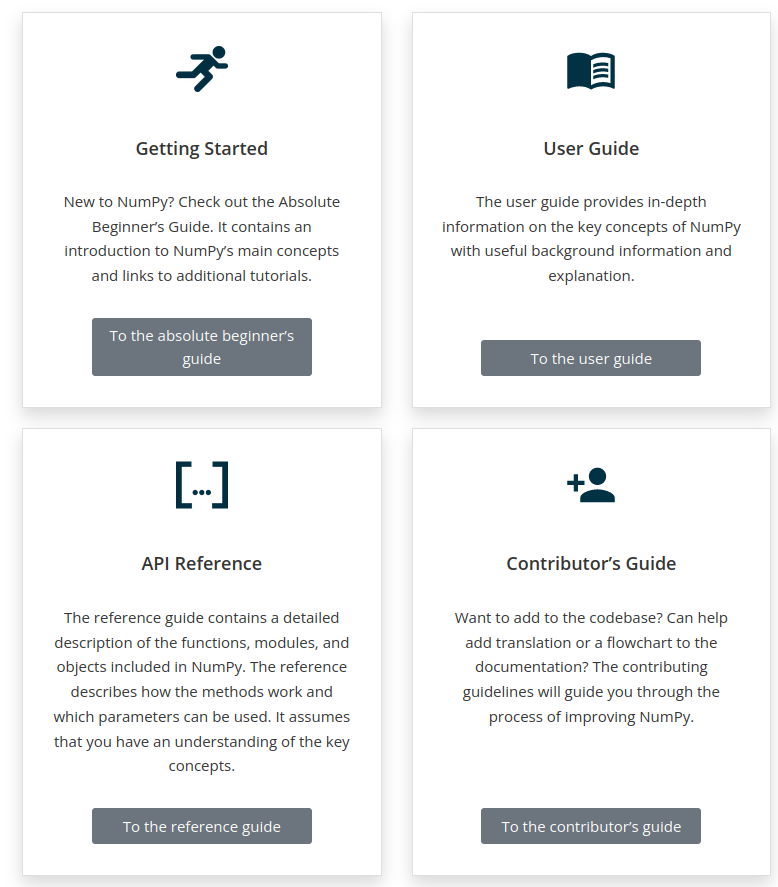
\includegraphics[width=\textwidth]{numpy-hierarchical-docs}
                \caption{
                    Numpy docs \href{https://numpy.org/doc/stable/}{starting page}.
                }
            \end{figure}

            % In general, it is convenient to document everything (e.g.\ with
            % docstrings), but the internals are for developers and
            % maintainability, not for users\footnote{
                % There should be a clear distinction, but they are both
                % important.
            % }.
            % \vspace*{10pt}
        \end{column}
    \end{columns}
\end{frame}

\begin{frame}{Home and Tutorials}
    \begin{columns}
        \begin{column}{0.5\textwidth}
            \vspace*{5pt}

            A good landing page is fundamental:
            \begin{itemize}
                \item a \textbf{unique reference} point
                \item communicate the \textbf{target audience}, and
                \item the scope and \textbf{goal} of the project
            \end{itemize}

            \begin{figure}
                \centering
                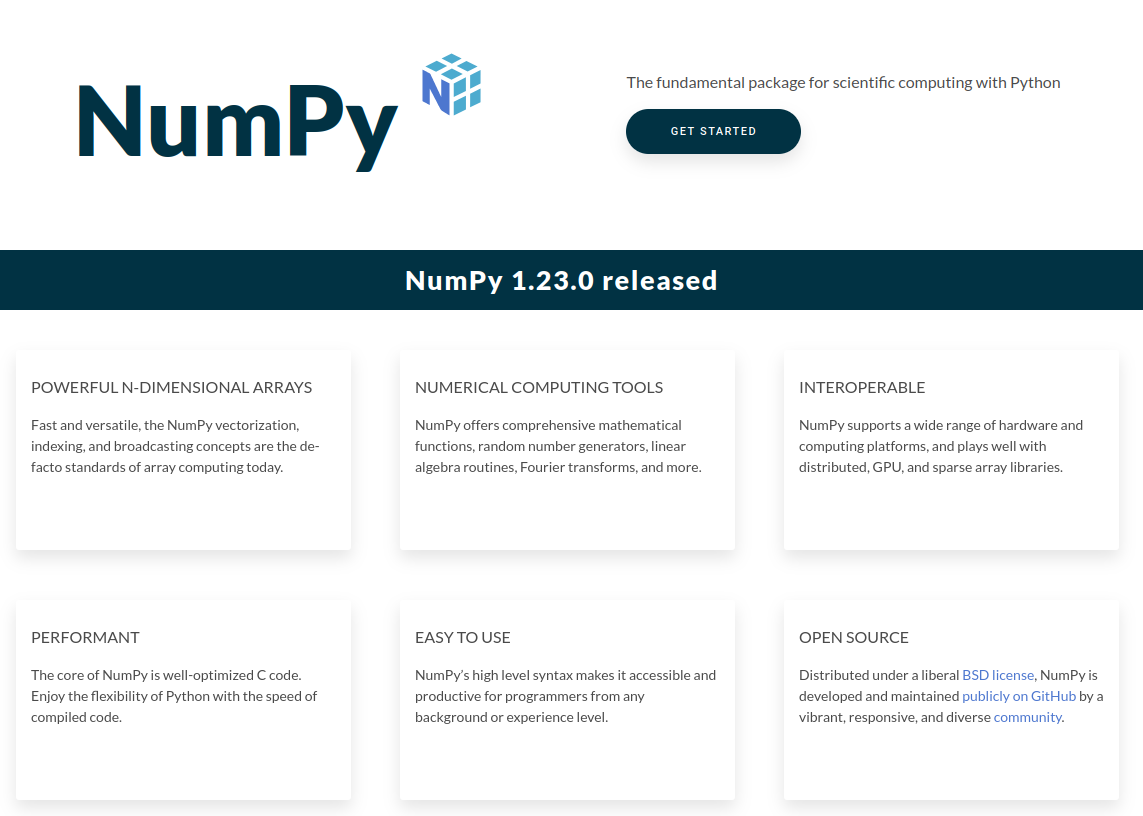
\includegraphics[width=0.8\textwidth]{numpy-home}
                \caption{Numpy \href{https://numpy.org/}{home}.}
            \end{figure}
            
            All the \textbf{relevant pointers} should be here, but only top
            level (think of a \textit{logarithmic navigation}).
        \end{column}
        \begin{column}{0.5\textwidth}
            \vspace*{10pt}

            \textbf{Tutorials} should be a \textit{\textbf{walk-through}}, the
            user has to know nothing but the initial problem.
            \vspace*{5pt}

            Jupyter notebooks are very useful, with explanations and outputs.
            \vspace*{5pt}

            \begin{figure}
                \centering
                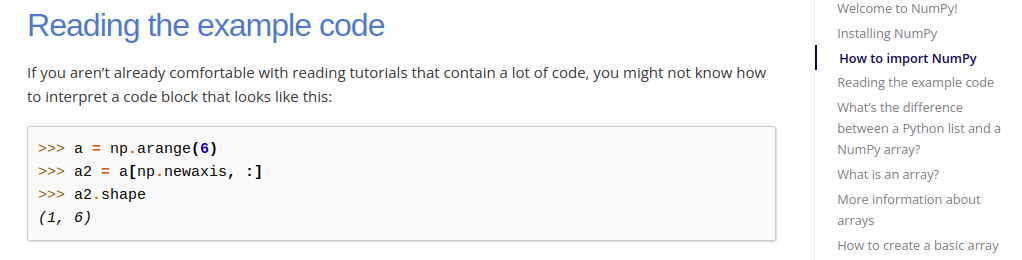
\includegraphics[width=0.9\textwidth]{numpy-abs-beginners}
                \caption{
                    Numpy
                    \href{https://numpy.org/doc/stable/user/absolute_beginners.html}{absolute
                    beginners} guide.
                }
            \end{figure}

            Consider to incrementally collect good examples. If easily
            discoverable they can be extremely useful.
            \vspace*{5pt}

            \begin{figure}
                \centering
                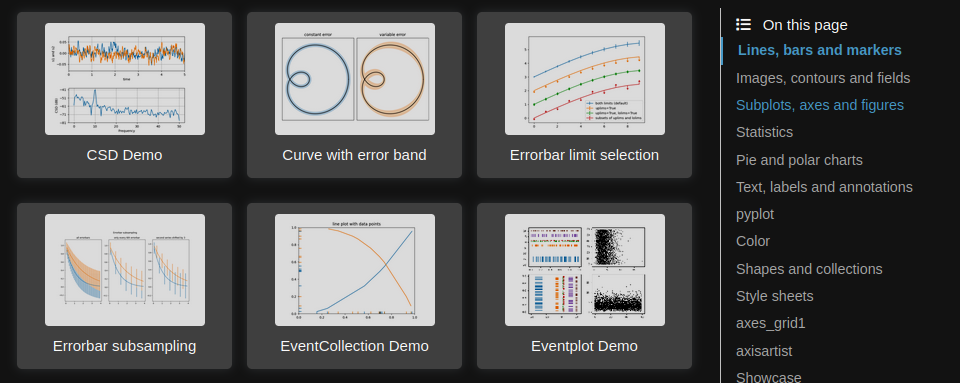
\includegraphics[width=0.8\textwidth]{matplotlib-gallery}
                \caption{
                    Matplotlib
                    \href{https://matplotlib.org/stable/gallery/}{gallery}
                }
            \end{figure}
        \end{column}
    \end{columns}
\end{frame}

\begin{frame}{Dependencies}
    \begin{columns}
        \begin{column}{0.5\textwidth}
            Another
        \end{column}
        \begin{column}{0.5\textwidth}
            \begin{figure}
                \centering
                \begin{tcolorbox}[size=tight,sharpish corners,boxrule=0mm]
                    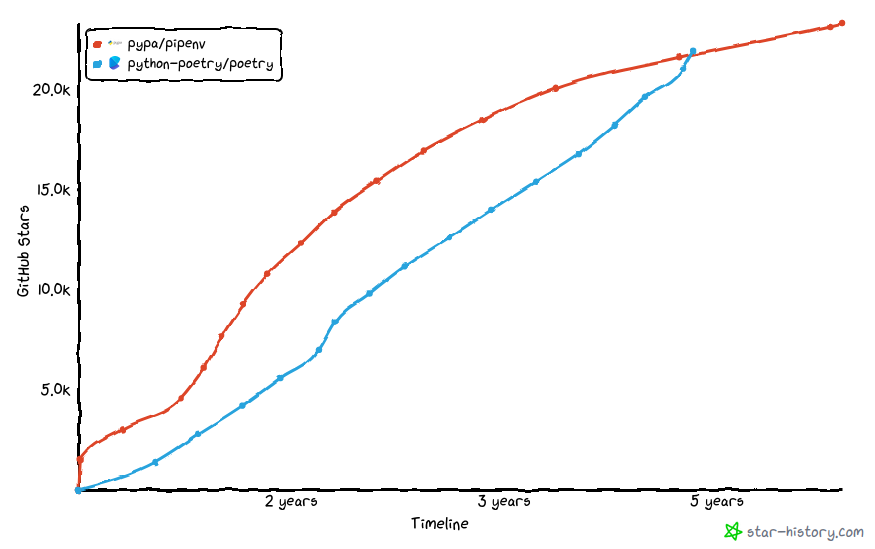
\includegraphics[width=\textwidth]{poetry-vs-pipenv}
                \end{tcolorbox}
                \caption{
                    Both a dependency managers comparison, and a good example
                    of trade-off: Pipenv is older, but Poetry has traction.
                }
            \end{figure}
        \end{column}
    \end{columns}
\end{frame}

\begin{frame}[standout]
    Thanks for your attention!
\end{frame}

\appendix

\begin{frame}{Template}
    \begin{columns}
        \begin{column}{0.5\textwidth}
            
        \end{column}
        \begin{column}{0.5\textwidth}
            
        \end{column}
    \end{columns}
\end{frame}

\begin{frame}[fragile]{Poetry tutorial \& references}
    \begin{columns}
        \begin{column}{0.1\textwidth}
        \end{column}
        \begin{column}{0.4\textwidth}
            Tutorial
            \begin{lstlisting}[language=bash,style=mystyle]
# install dependencies
poetry install
# add dependency
poetry add mypackage
# add dependency to given group
poetry add mypackage -G mygroup

# generate lockfile
poetry lock
# update dependencies
poetry update

# run command in environment
poetry run mycommand
# enter shell inside environment
poetry shell\end{lstlisting}
        \end{column}
        \begin{column}{0.4\textwidth}
            References
            \lipsum[1]
        \end{column}
        \begin{column}{0.1\textwidth}
        \end{column}
    \end{columns}
\end{frame}


\end{document}
